\documentclass[a4paper,12pt]{article}
\usepackage{outline}
\usepackage{pmgraph}
\usepackage[normalem]{ulem}
\usepackage{comment} % enables the use of multi-line comments (\ifx \fi)
\usepackage{lipsum} %This package just generates Lorem Ipsum filler text.
\usepackage{fullpage} % changes the margin
\usepackage{listings}
\usepackage{color}
\usepackage{mdframed}
\usepackage{listings}
\usepackage{amssymb}
\usepackage{amsmath}
\usepackage{graphicx}
\graphicspath{ {../screenshots/} }
\renewcommand{\lstlistingname}{Code Block}% Listing -> Algorithm
\renewcommand{\lstlistlistingname}{List of \lstlistingname s}% List of Listings -> List of Algorithms

\linespread{1.5}
%--------------------Indention
\setlength{\parindent}{15pt}
\lstset{frame=shadowbox, rulesepcolor=\color{white}}
\mdfsetup{frametitlealignment=\center}
\lstset{
  numbers=left,
  stepnumber=1,
  firstnumber=1,
  numberfirstline=true
}

\begin{document}
\section*{Objective}

  \hspace{15pt}The purpose of this lab was to expand on the students familiarity of sequential circuits
  by exposing them to the inner workings of a binary counter. The lab manual guided the students
  through desgining a binary up-counter using Verilog. Once designing was complete, the design
  will be synthesized onto the FPGA board using a student edited UCF file. Finally, the lab
  will conclude with two important use cases for binary counters, namely clock frequency division
  and I/O debouncing.

\section*{Design}
% The order is
% clock_divider.v
% 4 seperate clock signals image
% half_adder.v
% up_counter.v
% up countere image
% clock divider was edited so Count was 26 bits wide
% top_level.v
% top_level.ucf
% swich_bounce.v
% noDebounce.v
% withDebounce.v

  \lstinputlisting[language=Verilog,,caption=Clock Divider ]{../code/clock_divider.v}

  \lstinputlisting[language=Verilog,,caption=Half Adder ]{../code/half_adder.v}

  \lstinputlisting[language=Verilog,,caption=Up Counter ]{../code/up_counter.v}

  \lstinputlisting[language=Verilog,,caption=Top Level (Verilog) ]{../code/top_level.v}

  \lstinputlisting[language=Verilog,,caption=Top Level UCF ]{../code/top_level.ucf}

  \lstinputlisting[language=Verilog,,caption=Switch Bounce ]{../code/switch_bounce.v}

  \lstinputlisting[language=Verilog,,caption=No Debounce ]{../code/noDebounce.v}

  \lstinputlisting[language=Verilog,,caption=With Debounce ]{../code/withDebounce.v}

\section*{Results}

Measure and record the period of each clock signal using the green and yellow markers. Based
on your measurements, what frequency do you think the input (Experiment 1.4.b)
2. Open up the test bench file and try to understand what is going on. You should see that the test
bench produces a Clk signal. What is the frequency of that signal? (Exp 2.2.b)
3. You should also see that the test bench holds the counter in reset for a specific interval of time.
How long is that interval? (Exp 2.2.c)
4. After reset is de-asserted, the test bench holds the enable LOW for some amount of time before
allowing the counter to run. How long is this time period? (Exp 2.2.d)
5. What is this maximum count value and what signal in the waveform could we use to know
exactly when the counter is going to roll over? (Exp 2.2.f)
6. If we use a 50MHz clock to drive our frequency divider, what rate will the most significant bit
of the divider oscillate at? (Exp 2.3.a)
7. Copy the waveform on the scope into your lab write-up. (Exp 3.1.j)
8. Does the design work as intended? Why or why not? (Exp 3.2.f)

% Figure with caption
\newpage
\begin{figure}[h]
  \begin{center}
    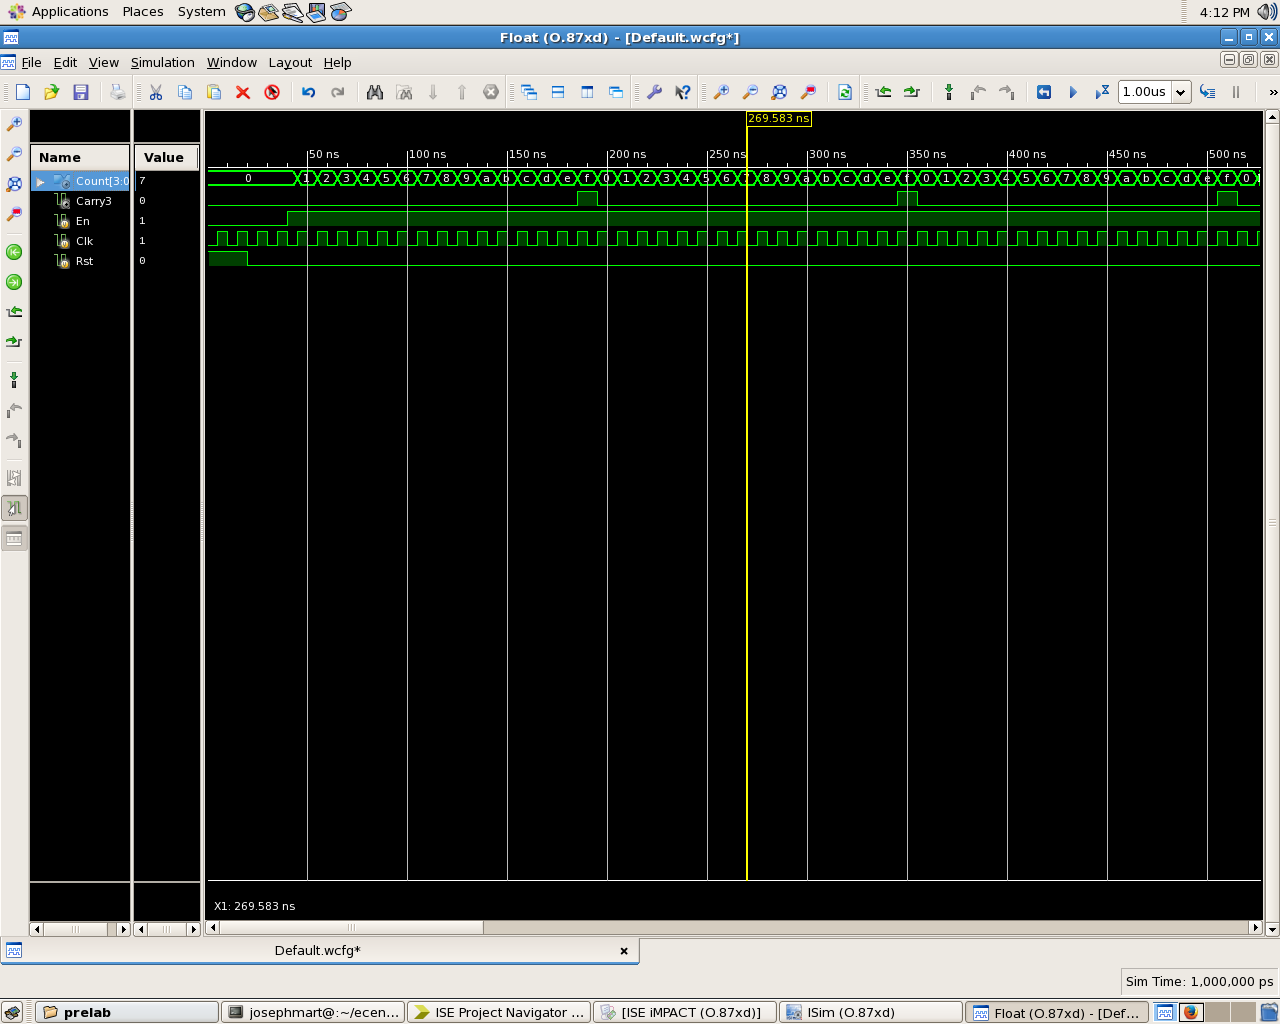
\includegraphics[scale=.1]{2_2_e.png}
    \caption{\textit{2-Bit 2:1 MUX Plots}}
  \end{center}
\end{figure}
\newpage
\begin{figure}[h]
  \begin{center}
    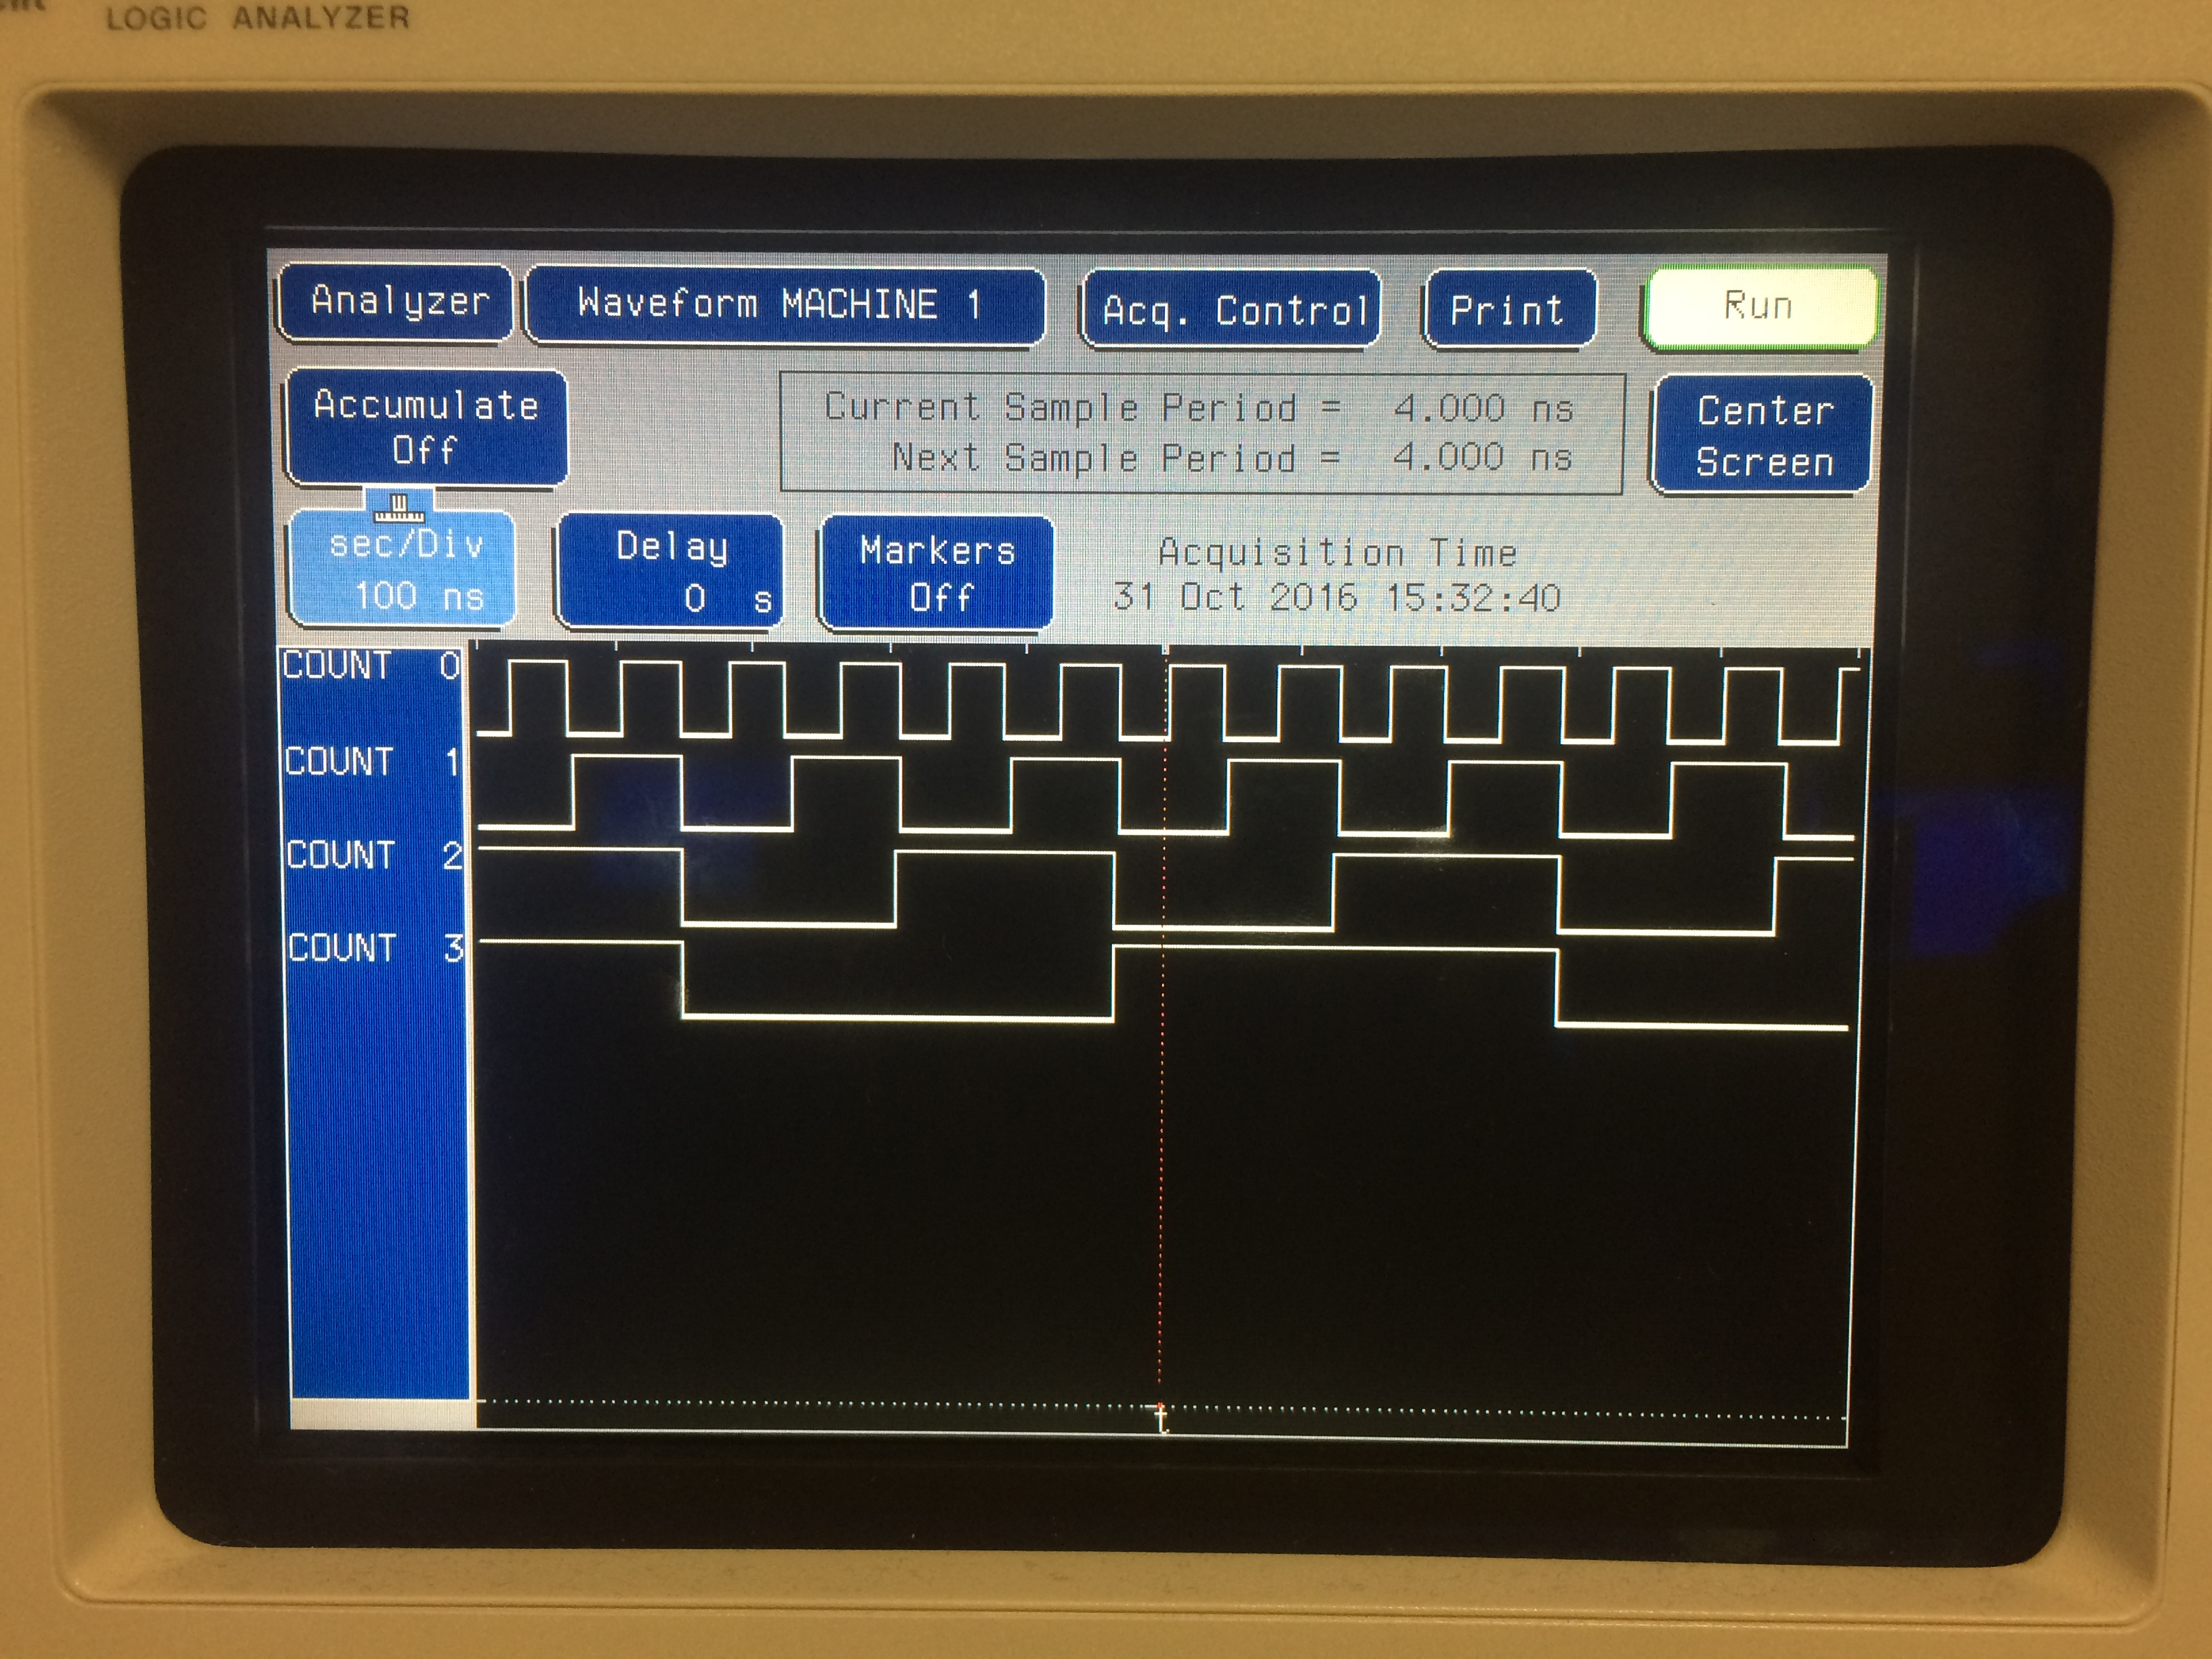
\includegraphics[scale=.1]{IMG_8620.JPG}
    \caption{\textit{2-Bit 2:1 MUX Plots}}
  \end{center}
\end{figure}
\newpage
\begin{figure}[h]
  \begin{center}
    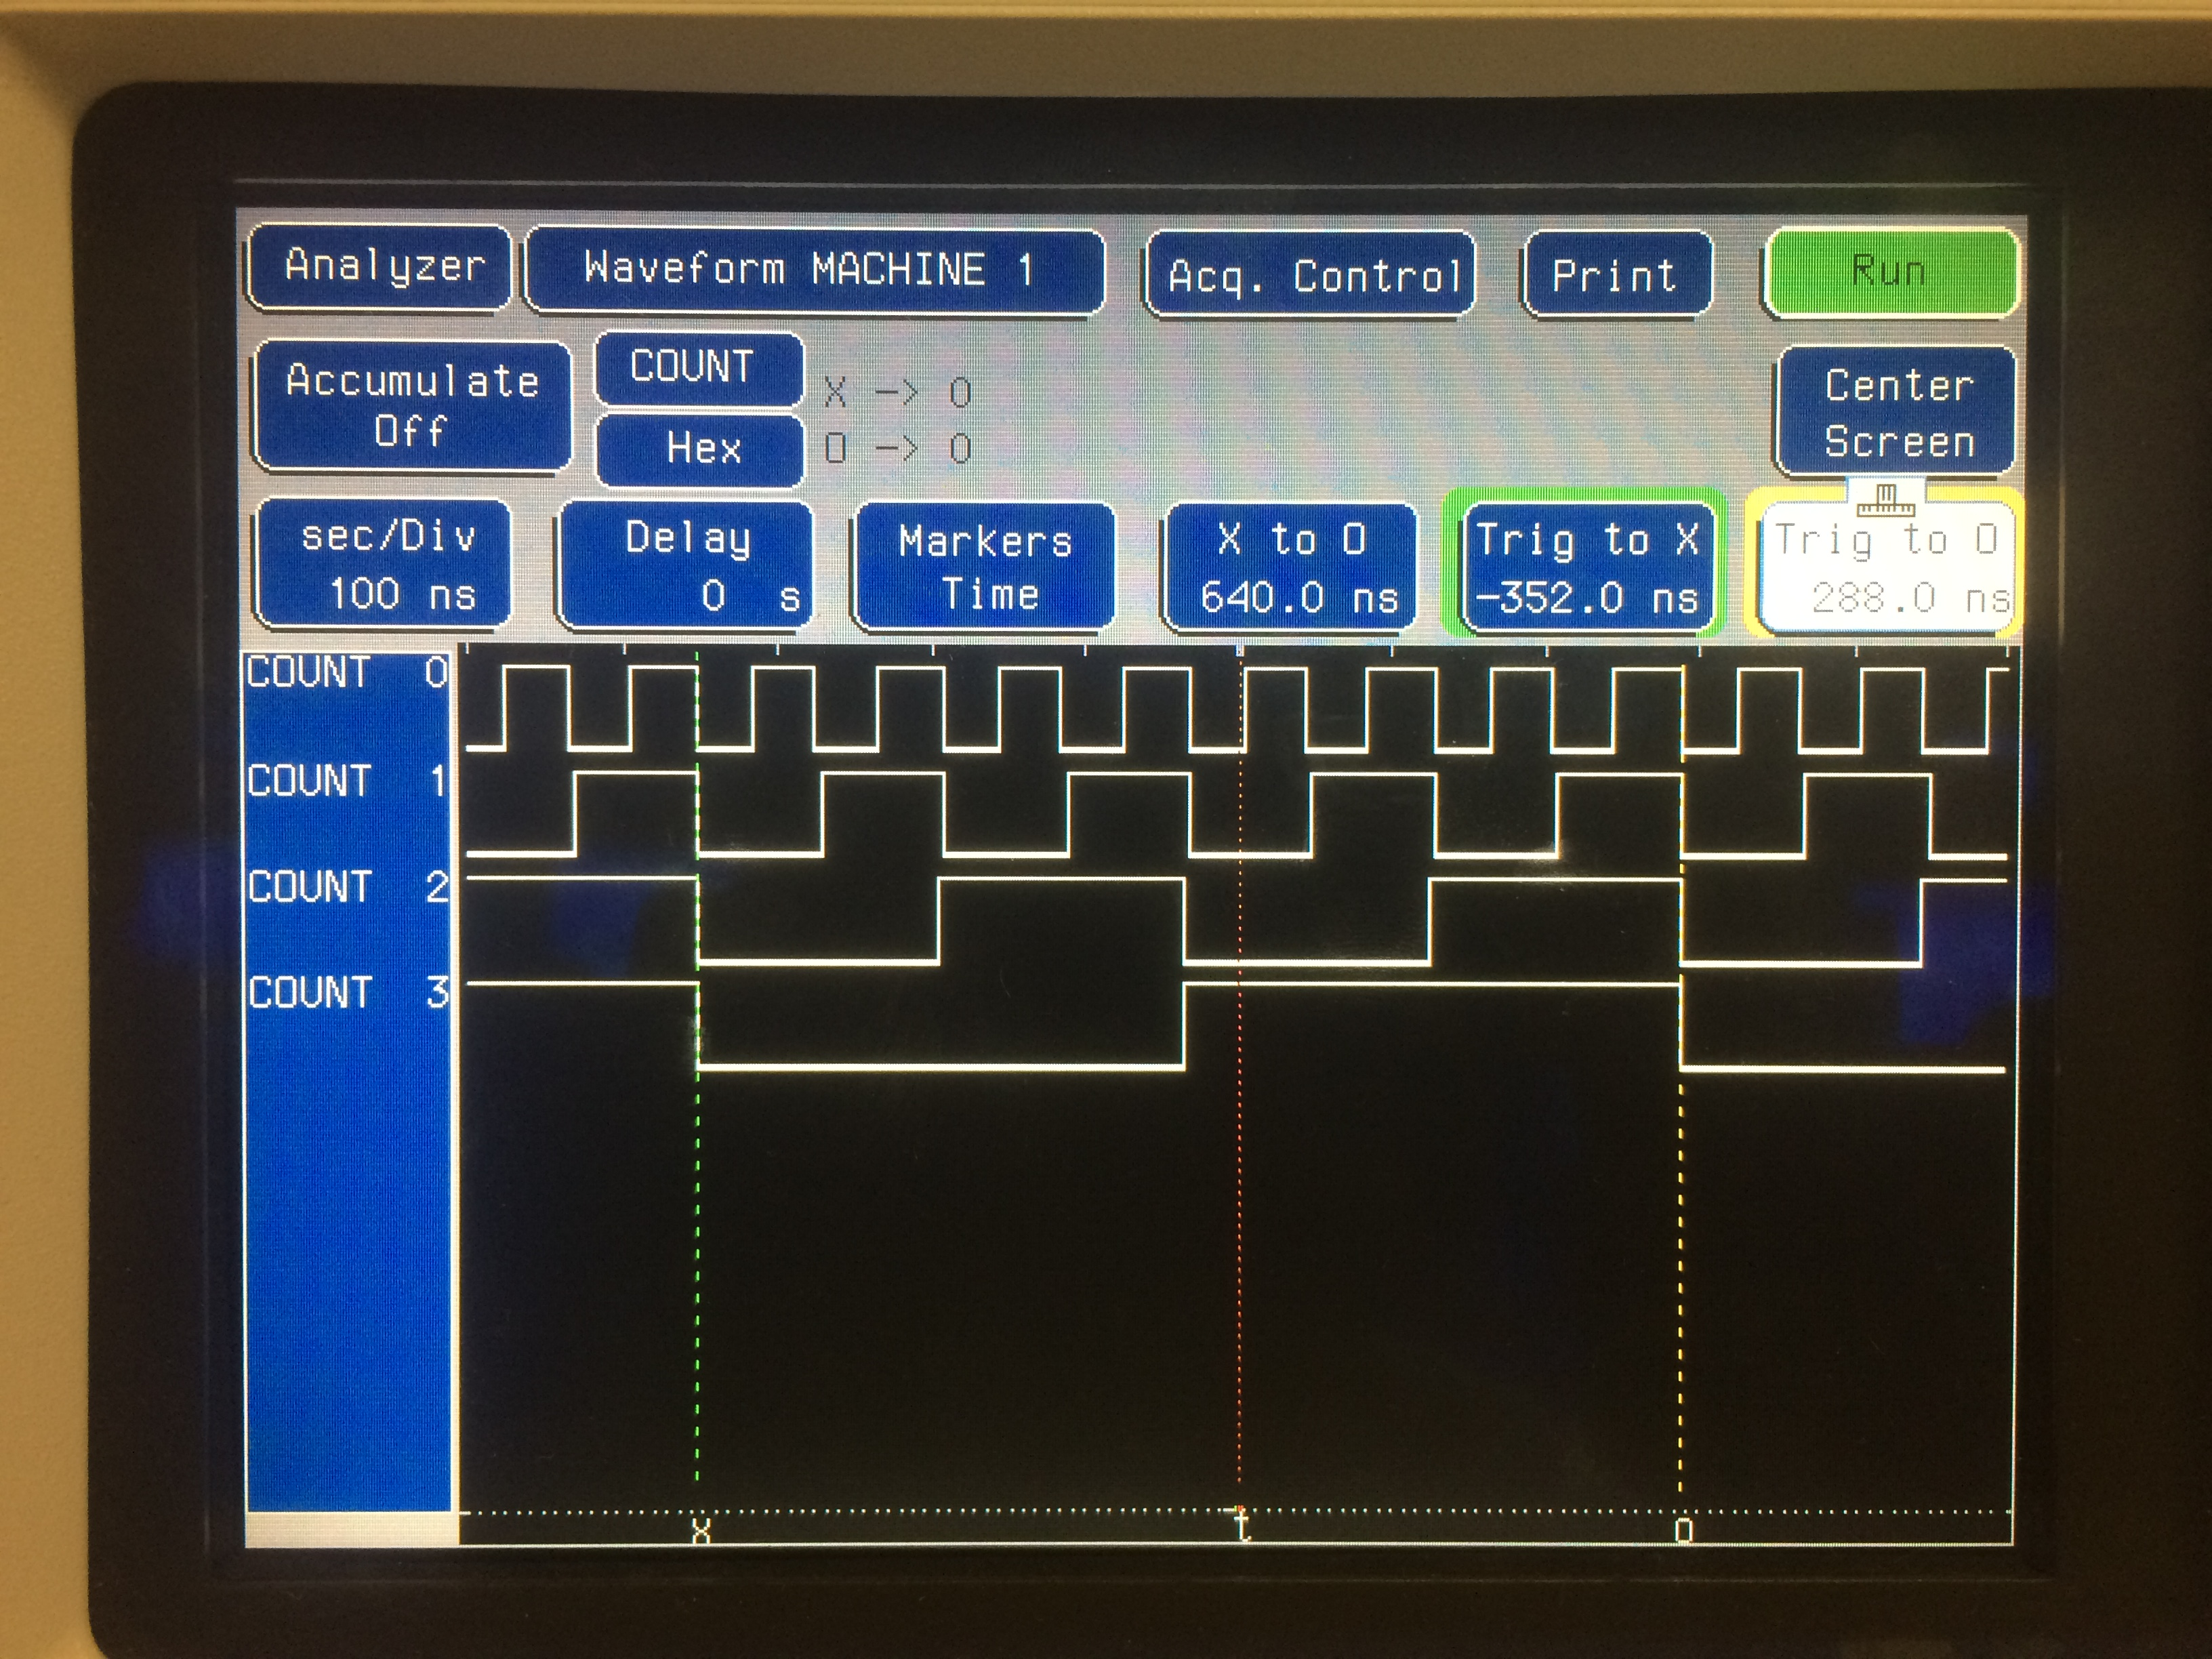
\includegraphics[scale=.1]{IMG_8621.JPG}
    \caption{\textit{2-Bit 2:1 MUX Plots}}
  \end{center}
\end{figure}
\newpage
\begin{figure}[h]
  \begin{center}
    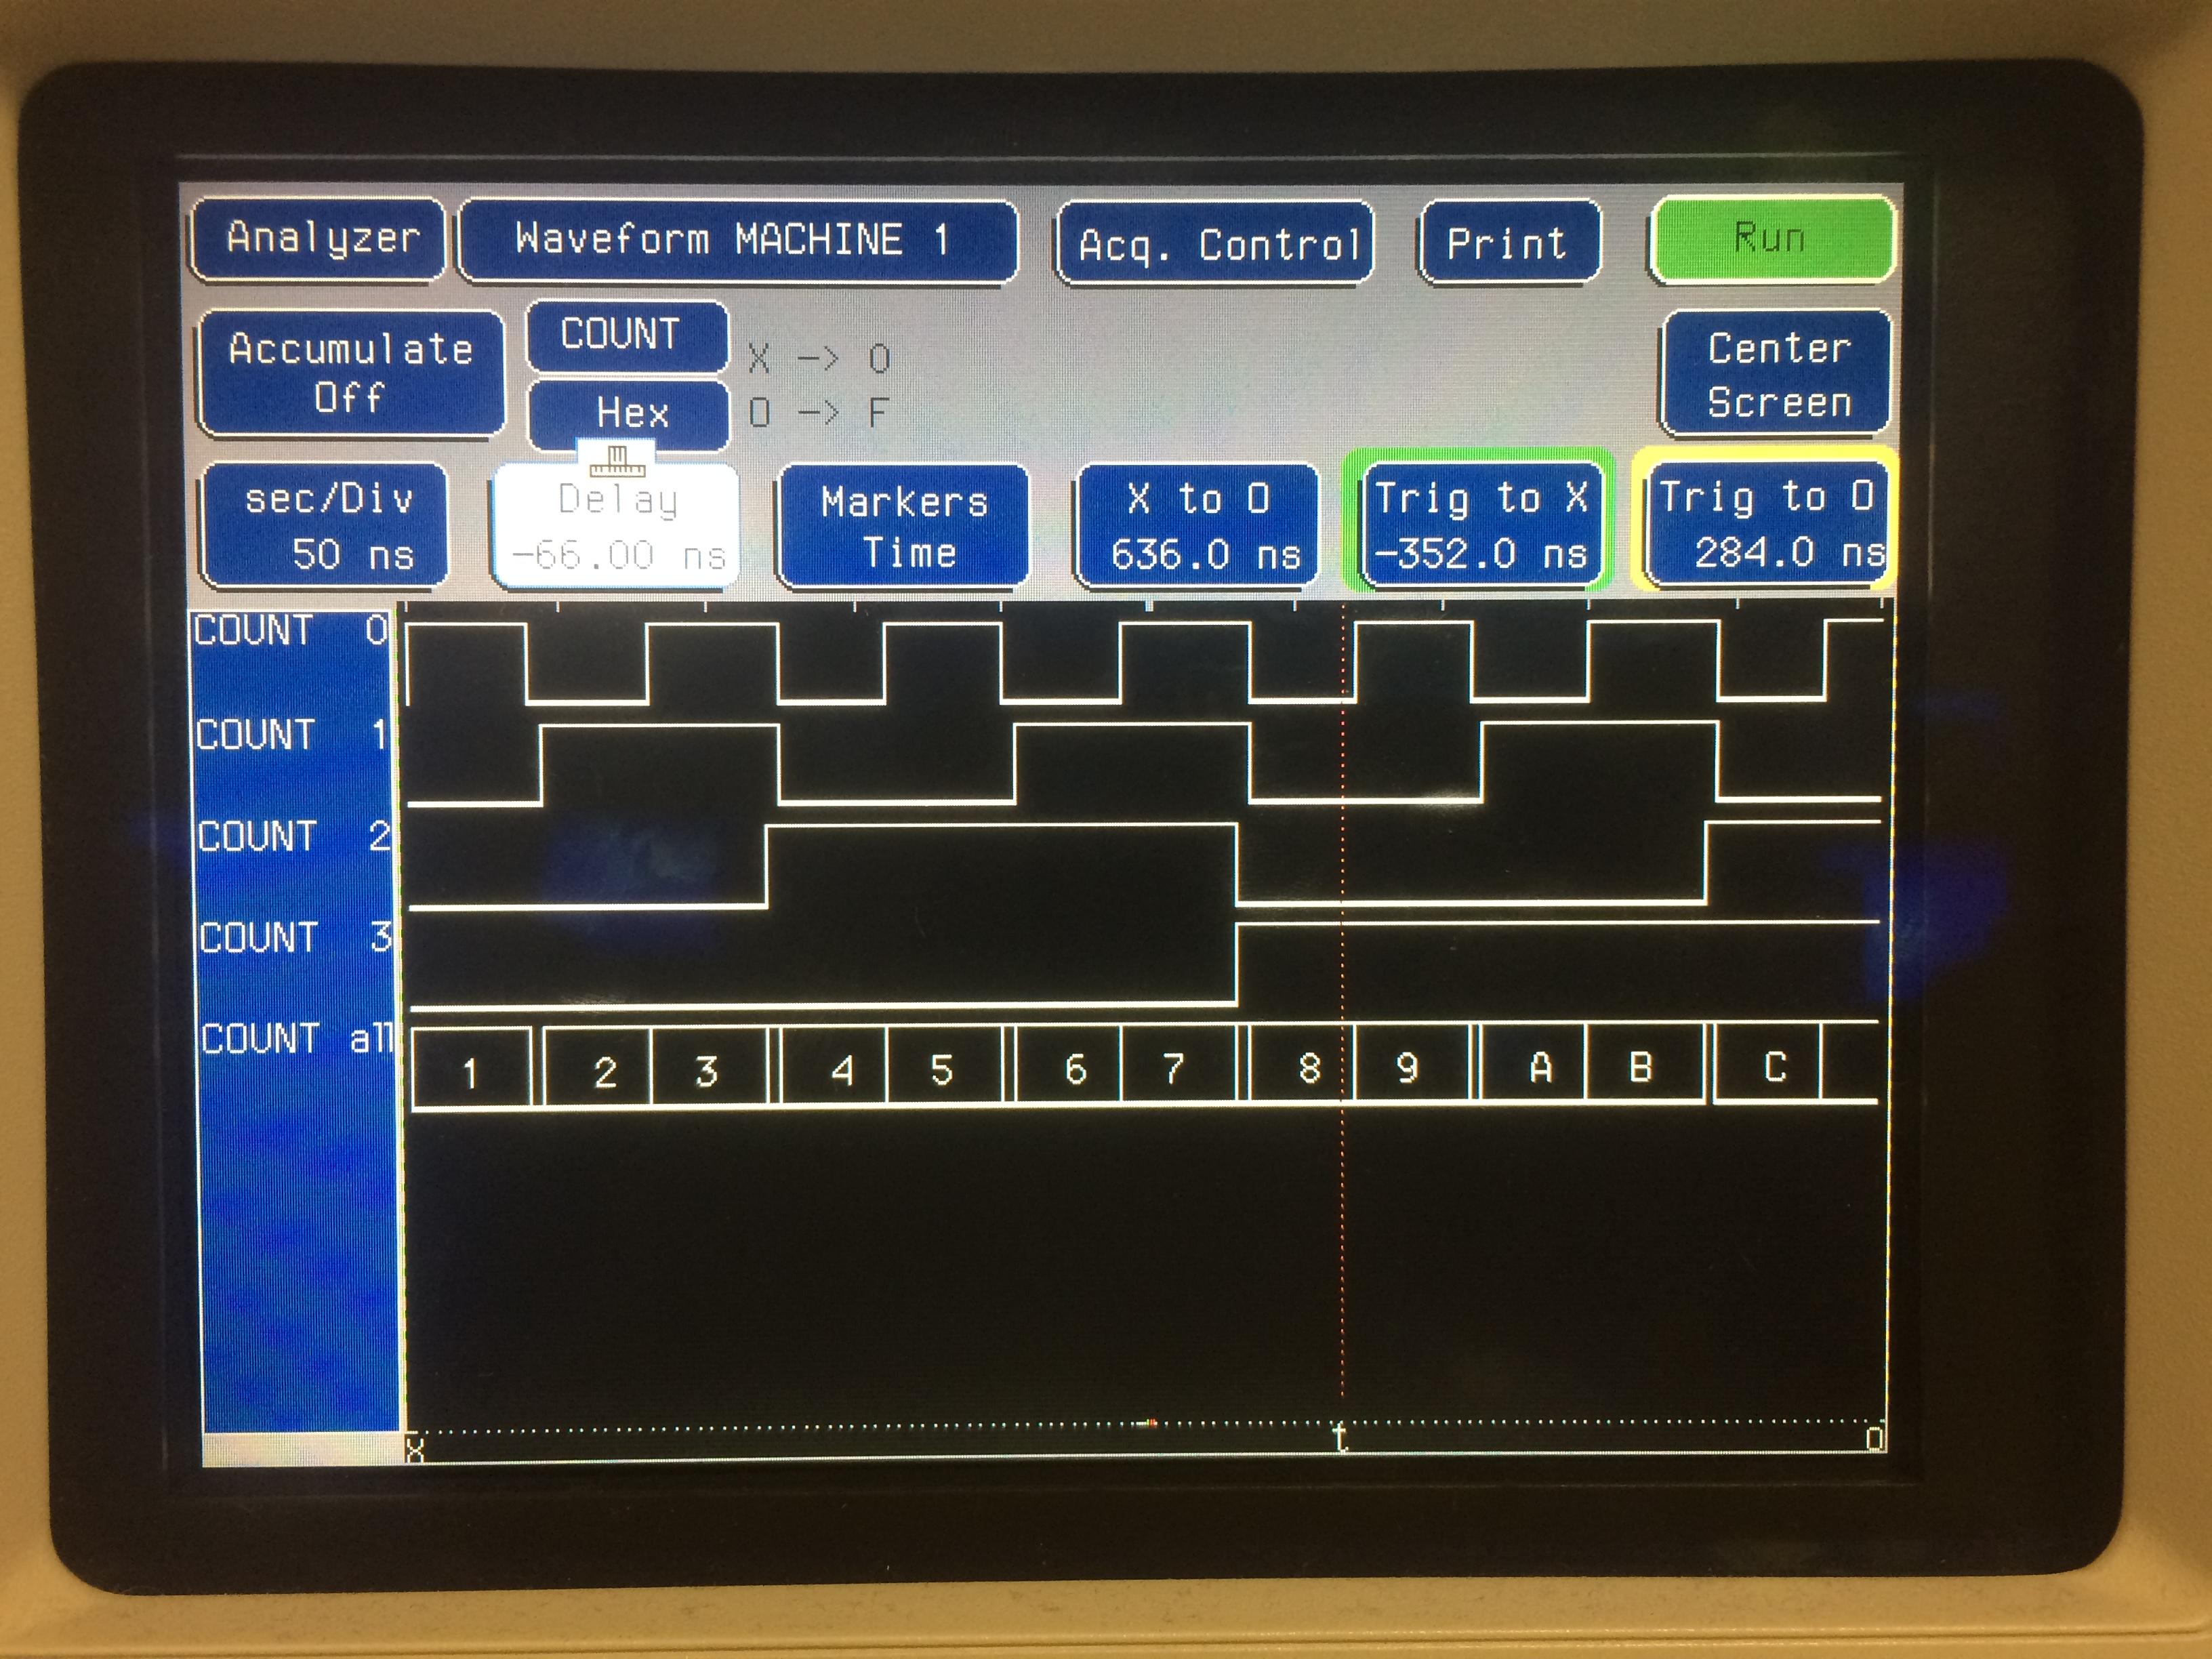
\includegraphics[scale=.1]{IMG_8622.JPG}
    \caption{\textit{2-Bit 2:1 MUX Plots}}
  \end{center}
\end{figure}
\newpage
\begin{figure}[h]
  \begin{center}
    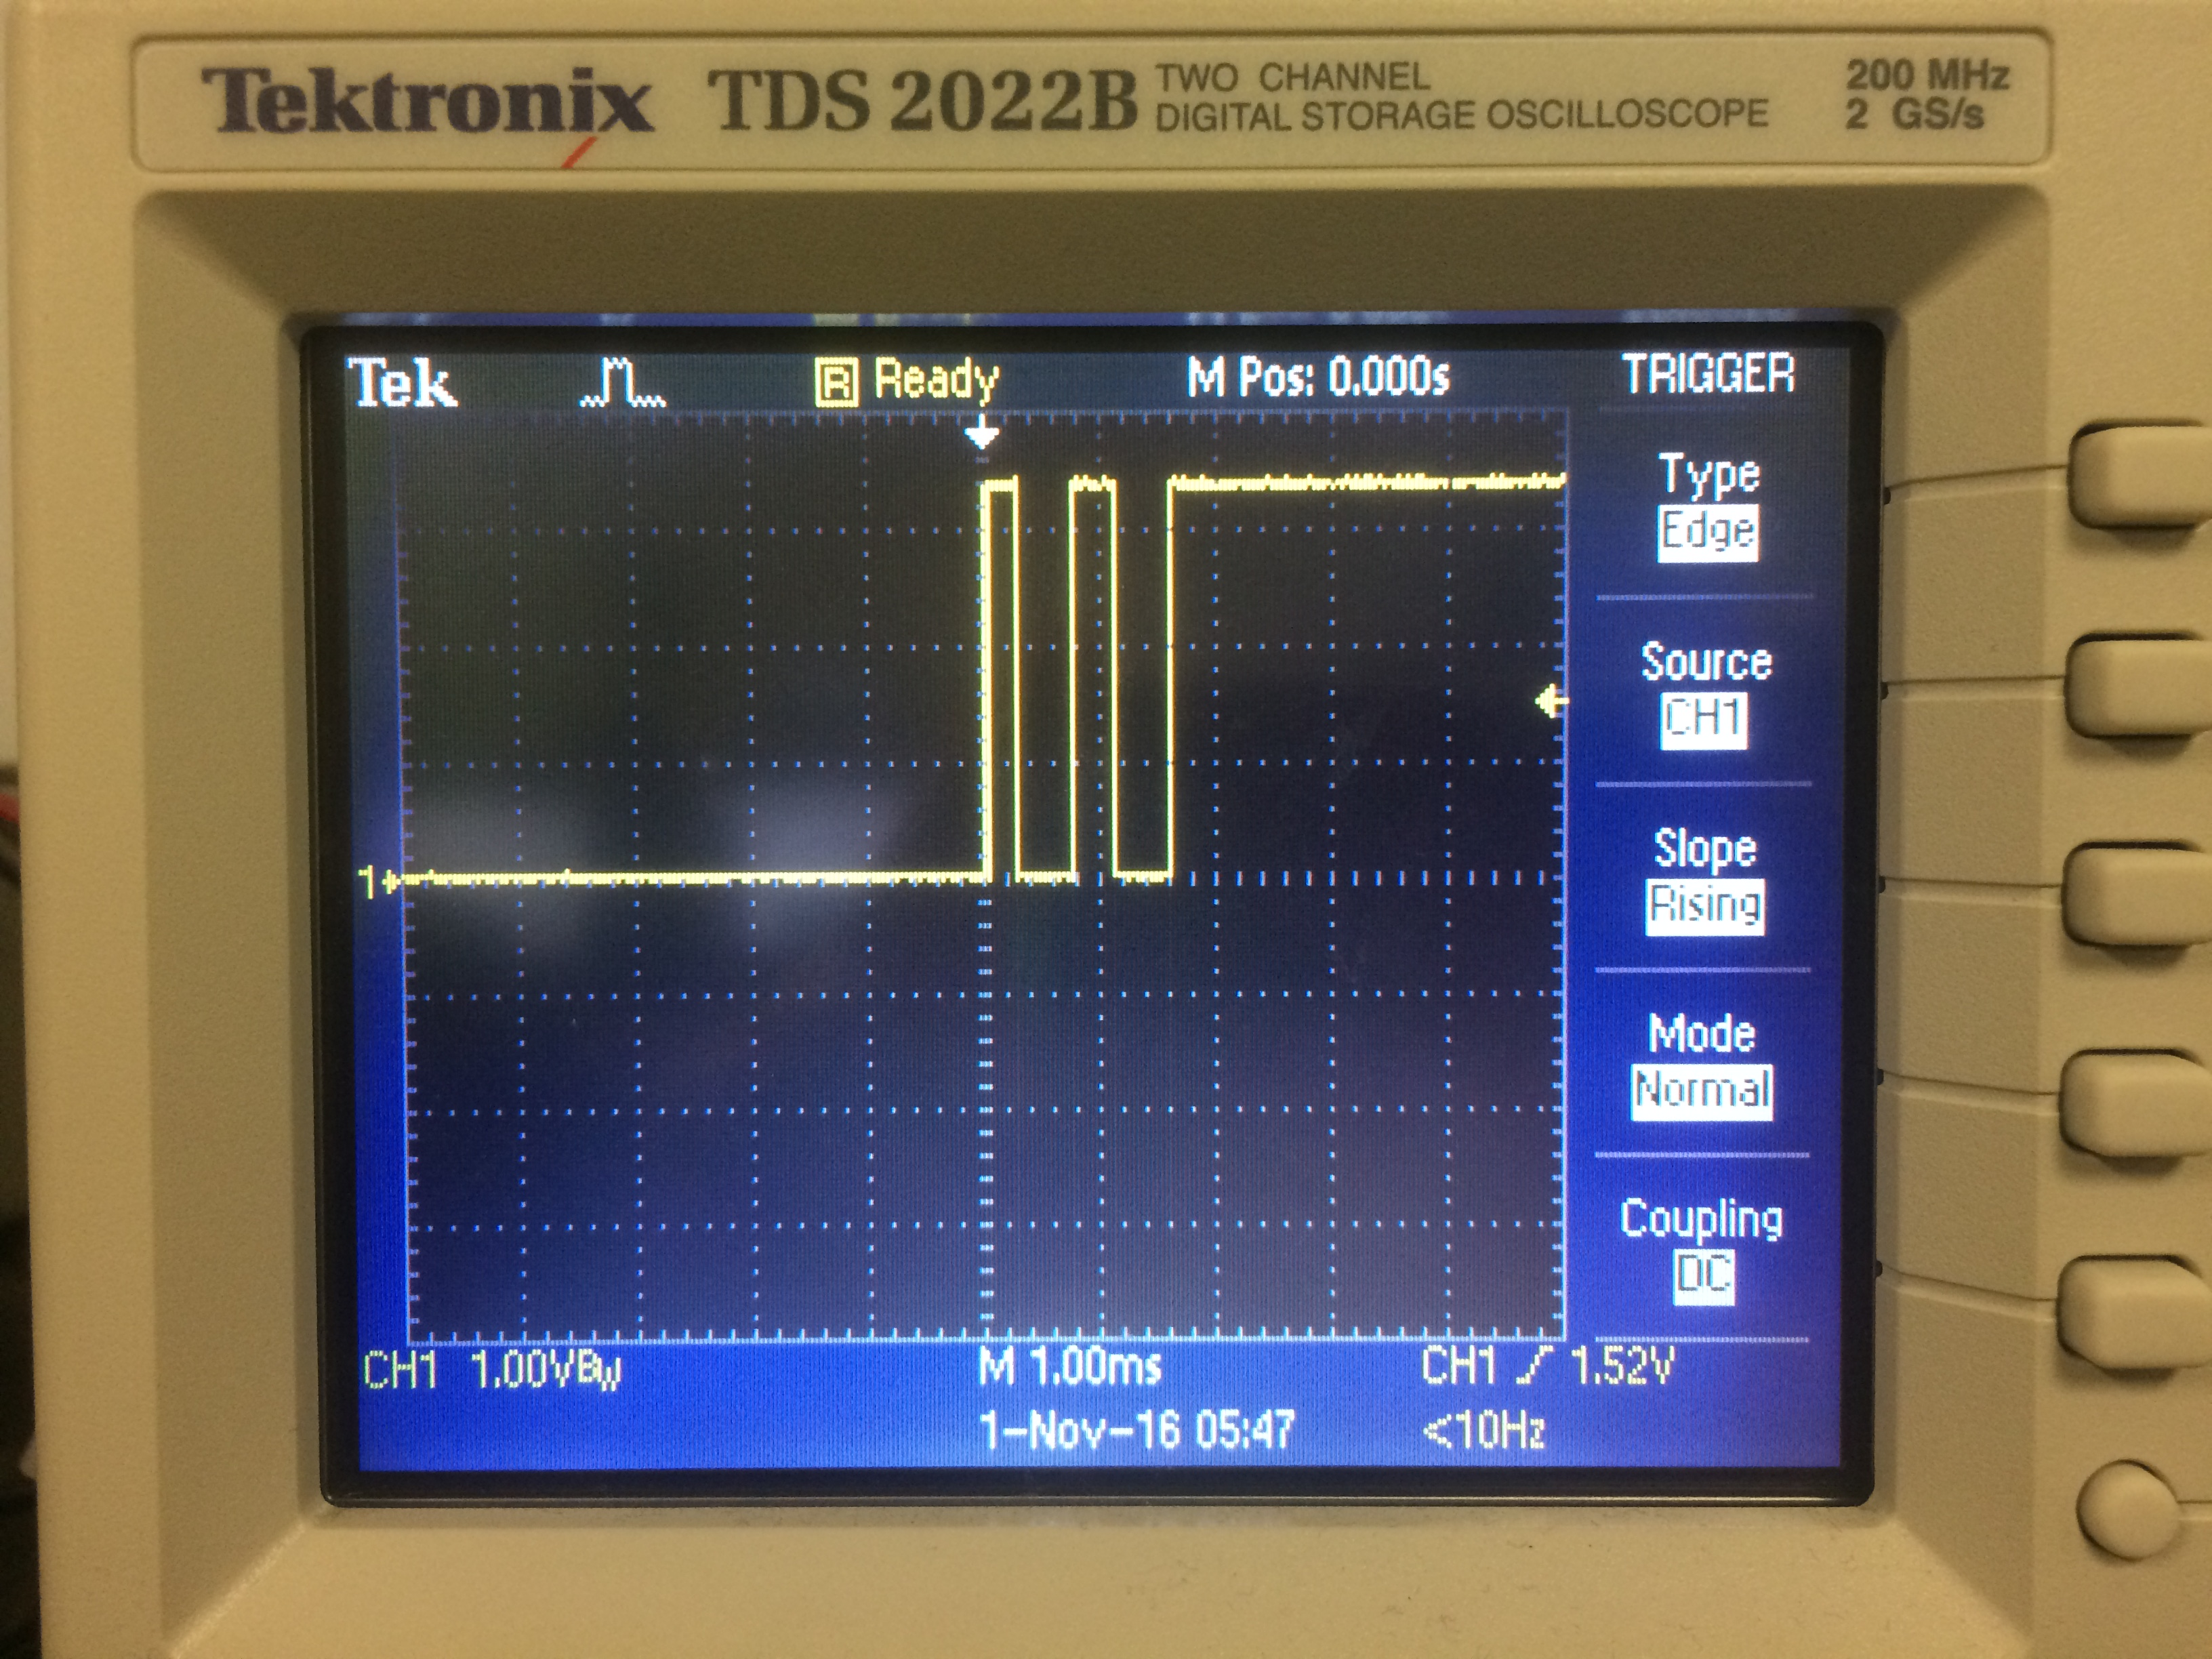
\includegraphics[scale=.1]{IMG_8624.JPG}
    \caption{\textit{2-Bit 2:1 MUX Plots}}
  \end{center}
\end{figure}
\newpage
\begin{figure}[h]
  \begin{center}
    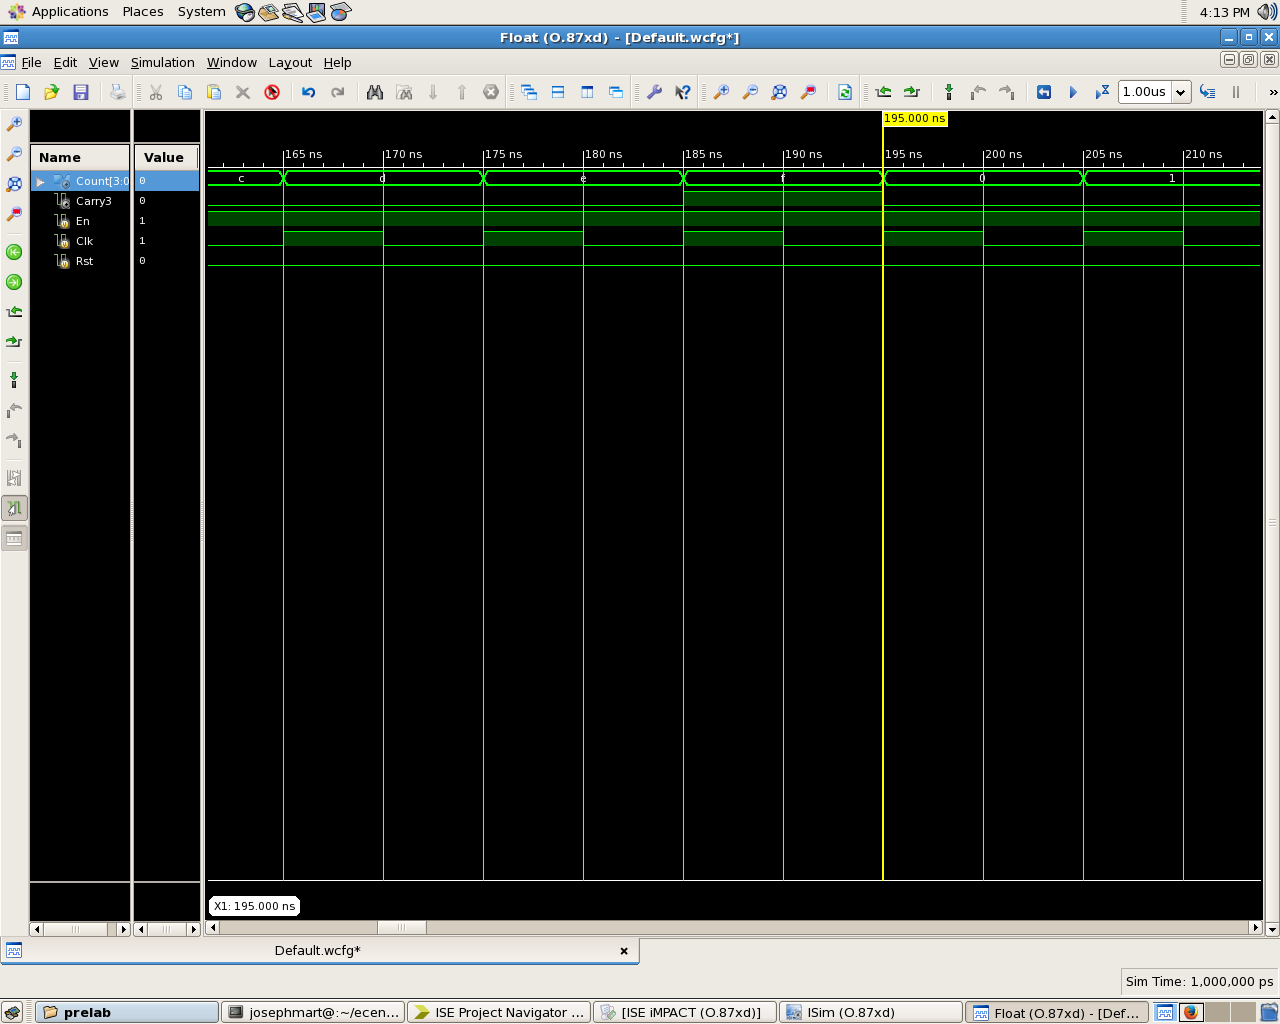
\includegraphics[scale=.1]{RollOver.png}
    \caption{\textit{2-Bit 2:1 MUX Plots}}
  \end{center}
\end{figure}
\newpage
\begin{figure}[h]
  \begin{center}
    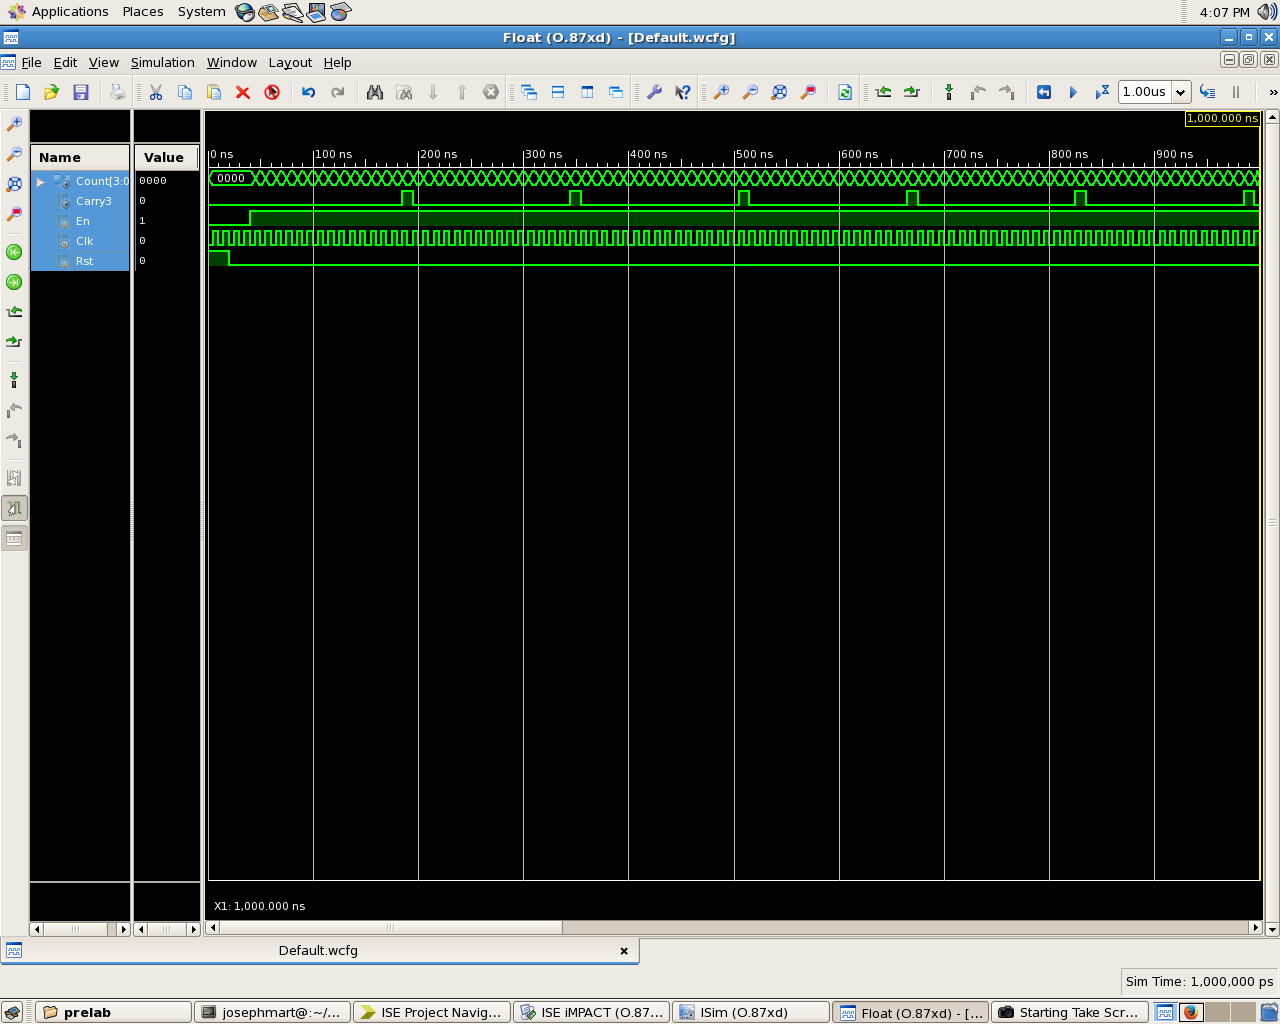
\includegraphics[scale=.1]{up_Count_waveform.png}
    \caption{\textit{2-Bit 2:1 MUX Plots}}
  \end{center}
\end{figure}

\section*{Conclusions}


\section*{Questions}

\begin{enumerate}
  \item \textbf{Include the source code with comments for all modules in lab. You do not have to include test bench
  code. Code without comments will not be accepted!}

  \textit{In the report.}
  
  \item \textbf{Include any UCFs that you wrote or modified.}

  \textit{In the report.}
  
  \item \textbf{Include screenshots of all waveforms captured during simulation in addition to the test bench console
  output for each test bench simulation.}

  \textit{In the report.}

  \item \textbf{Answer all questions throughout the lab manual.}

  \item \textbf{Measure and record the period of each clock signal using the green and yellow markers. 
  Based on you measurements, what frequency do you think the input clock is running at?}
  
  COUNT0 - 80 ns \\
  COUNT1 - 160 ns \\
  COUNT2 - 320 ns \\
  COUNT3 - 640 ns \\
  CLock in should be 40 resulting in a frequency of 25 MHz
  
  \item \textbf{Open up the test bench file and try to understand what is going on. You should see that the test
  bench produces a Clk signal. What is the frequency of that signal?}
  
  In the test bench, the clock signal is held for 5 ns high and then 5 ns low which would result in a 10 ns cycle. The frequency would then be 100 MHz
  
  \item \textbf{You should also see that the test bench holds the counter in reset for a specific interval of time. How long is that interval?}
  
  The interval is 20 ns
  
  \item \textbf{After reset is de-asserted, the test bench holds the enable LOW for some amount of time before 
  allowing the counter to run. How long is this time period?}
  
  This time period is 20 ns.
  
  \item \textbf{What is this maximum count value and what signal in the waveform could we use to know
  exactly when the counter is going to roll over?}
  
  The maximum count value is f in hexadecimal or 15 in decimal. Whenever Carry3 was HIGH, Count was a max, on the downward edge of Carry3, the Count would reset/roll over
  
  \item \textbf{If we use a 50MHz clock to drive our frequency divider, what rate will the most significant bit
  of the divider oscillate at?}
  
  $f_2 = \dfrac{f_1}{2^n} = \dfrac{50 mHz}{2^{26}} = 0.745 Hz$
  
  \item \textbf{Make note in you lab write-up how the switches affected the LED outputs.}
  
  The switches slowed down the rate at which the LEDs would count up. The fastest counting up would occur when none of the switches were toggled. The slowest would occur when both switches were toggled. This is due to the how the switches were interpreted into binary. There were two switches $S_0$ and $S_1$ where $S_0$ was of least importance. As the binary value of the switches went up, the speed of the LEDs would slow down.
  
  \item \textbf{Make a note in you lab write up of what what is described in these (Switch Bounce) files.}
  
  It connects J10 to the B4 input on the board. It also connects center to V16 (big center button) on the board.

  \item \textbf{NoDebounce. Does the design work as intended?}
  
  The LEDs are a little glitchy because of multiple rising edges due to electrical chatter. 
  
  \item \textbf{Explain the operation of the circuit described in withDebounce.v}
  
  The input wire goes into two flip flops in order to synchronize the signal and eliminate electrical chatter. Then the signal goes into a binary counter. The LEDs correctly 
  incremented based on the number of times the button was pressed.     
  
\end{enumerate}

\section*{Student Feedback}

\begin{enumerate}
  \item \textbf{What did you like most about the lab assignment and why? What did you like least about it and why?}
  
  In this lab, working with a partner proved to be very beneficial. Our ground circuit on the Logic Analyzer was faulty.

  \item \textbf{Were there any section of the lab manual that were unclear? If so, what was unclear? Do you have any suggestions for improving the clarity?}

  The lab manual was clear in this lab contrary to previous labs.

  \item \textbf{What suggestions do you have to improve the overall lab assignment?}
  
  Better equipment.

\end{enumerate}

\ifx
\begin{thebibliography}{1}
\bibitem{Verilog} Charles Kime \& Thomas Kaminski  \emph{Logic and Computer Design Fundamentals} \\ \hspace{15pt}\textit{http://www.cs.bilkent.edu.tr/~will/courses/CS223/Verilog/LCDF3_Verilog_Ch_4.pdf}
\end{thebibliography}

\section*{Attachments}
%Make sure to change these
Lab Notes, HelloWorld.ic, FooBar.ic
%\fi %comment me out

\begin{thebibliography}{9}
\bibitem{Verilog} Charles Kime & Thomas Kaminski  \emph{Logic and Computer Design Fundamentals} \textit{http://www.cs.bilkent.edu.tr/~will/courses/CS223/Verilog/LCDF3_Verilog_Ch_4.pdf}
\end{thebibliography}

%How to cite
Put your Problem statement here! Example of a Citation\cite[p.219]{Robotics}. Here's Another Citation\cite{Flueck}
\fi
\end{document}
